\documentclass[conference]{IEEEtran}
\usepackage{cite}
\usepackage{amsmath,amssymb,amsfonts}
\usepackage{algorithmic}
\usepackage{graphicx}
\usepackage{textcomp}
\usepackage{xcolor}
\usepackage{booktabs}
\usepackage{float}

% Title and Author
\title{Statistical Inference on Personal Health Data:\\ The Effect of Physical Activity on REM Sleep}

\author{\IEEEauthorblockN{Yiğit Ateş}
\IEEEauthorblockA{\textit{Institute for Data Science \& Artificial Intelligence} \\
\textit{Boğaziçi University}\\
Istanbul, Turkey \\
2025776009}
}

\begin{document}

\maketitle

\begin{abstract}
This project investigates the relationship between physical activity (daily step count) and REM sleep duration using personal health data collected over a period of fourteen months. Exploratory data analysis (EDA) revealed distinct temporal patterns, including a ``Social Jetlag'' phenomenon characterized by reduced sleep on Mondays and compensatory rebound on Saturdays. The daily REM sleep duration was found to follow a Normal distribution, validated by the Kolmogorov-Smirnov (KS) test. Parameter estimation was conducted using Maximum Likelihood Estimation (MLE), Method of Moments (MoM), and Bayesian methods. A one-sample t-test confirmed that the subject's average daily REM sleep significantly differs from the physiological benchmark of 1.5 hours, specifically exceeding it. Finally, a linear regression model demonstrated a statistically significant, albeit weak, positive correlation between daily step count and REM sleep duration.
\end{abstract}

\begin{IEEEkeywords}
statistical inference, exploratory data analysis, regression, hypothesis testing, sleep, rem sleep, physical activity
\end{IEEEkeywords}

\section{Introduction}
Sleep quality is a critical component of overall health, with Rapid Eye Movement (REM) sleep playing a vital role in memory consolidation and emotional processing. With the advent of wearable technology, it has become easier to track personal physiological metrics.

The objective of this project is to apply statistical inference techniques to real-world data to answer two key questions:
\begin{enumerate}
    \item Does the daily REM sleep duration follow a specific probability distribution?
    \item Is there a significant relationship between physical exertion (measured by step count) and the duration of REM sleep obtained the subsequent night?
\end{enumerate}

\section{Dataset and Preprocessing}
The dataset consists of 247 sleep observations collected between October 2024 and December 2025 using a Samsung Galaxy Watch.

\subsection{Temporal Definitions}
To avoid ambiguity, it is crucial to define the temporal assignment of sleep records. In this analysis, a "sleep record" is assigned to the day on which the subject wakes up.
\begin{itemize}
    \item \textbf{Example:} Sleep occurring between Sunday 23:00 and Monday 07:00 is recorded as \textit{Monday's} sleep duration.
    \item Consequently, behavioral factors described as "Sunday Night Procrastination" will manifest statistically in the \textit{Monday} column.
\end{itemize}

\subsection{Data Characteristics}
The dataset spans over a year, capturing different seasonal and life-stage variations. Table \ref{tab:combined_stats} presents the monthly descriptive statistics for both REM sleep duration and physical activity.

\begin{table}[H]
\centering
\caption{Monthly Statistics: REM Sleep vs. Step Count}
\label{tab:combined_stats}
\resizebox{\columnwidth}{!}{%
\begin{tabular}{@{}lcccccc@{}}
\toprule
 & \multicolumn{3}{c}{\textbf{REM Sleep Hours}} & \multicolumn{3}{c}{\textbf{Step Count}} \\ 
\cmidrule(lr){2-4} \cmidrule(lr){5-7}
Year-Month & N & Mean & Std & N & Mean & Std \\ \midrule
2024-10 & - & - & - & 30 & 5,478 & 4,046 \\
2024-11 & 29 & 1.90 & 0.59 & 30 & 7,732 & 3,940 \\
2024-12 & 26 & 1.72 & 0.40 & 31 & 7,875 & 4,502 \\
2025-01 & 15 & 1.66 & 0.56 & 31 & 6,780 & 4,181 \\
2025-02 & 8  & 1.65 & 0.35 & 28 & 7,768 & 4,498 \\
2025-03 & 4  & 1.98 & 0.30 & 31 & 6,954 & 4,377 \\
2025-04 & 20 & 1.54 & 0.38 & 30 & 6,854 & 4,132 \\
2025-05 & 19 & 1.47 & 0.44 & 30 & 6,645 & 3,781 \\
2025-06 & 18 & 1.70 & 0.44 & 30 & 9,379 & 5,420 \\
2025-07 & 21 & 1.75 & 0.24 & 31 & 8,618 & 4,393 \\
2025-08 & 20 & 1.64 & 0.53 & 31 & 8,197 & 5,239 \\
2025-09 & 18 & 1.77 & 0.48 & 30 & 9,944 & 5,126 \\
2025-10 & 20 & 1.78 & 0.42 & 31 & 9,559 & 5,339 \\
2025-11 & 20 & 1.56 & 0.60 & 29 & 9,763 & 5,102 \\
2025-12 & 10 & 1.86 & 0.38 & 13 & 10,716 & 4,746 \\ \bottomrule
\end{tabular}%
}
\end{table}

\subsection{Preprocessing}
To ensure a consistent unit of analysis, multiple sleep sessions (naps) occurring within the same day were aggregated to produce a single total sleep and REM duration for each date.

\subsection{Variables}
\begin{itemize}
    \item \textbf{Dependent Variable ($Y$):} \texttt{daily\_rem\_hours} (Continuous). Calculated as the total minutes of REM sleep divided by 60.
    \item \textbf{Independent Variable ($X$):} \texttt{count} (Discrete). The total number of steps taken during the day.
\end{itemize}

\subsection{Data Alignment}
A critical preprocessing step involved aligning the timelines of the two datasets. Sleep data is timestamped by the "wake-up" time (end time), whereas step data is timestamped by the day the activity occurred. To analyze the effect of daily activity on that night's sleep, the step count from Day $T$ was merged with the sleep record ending on Day $T+1$.

After filtering for missing values and aligning dates, the final dataset contained $N=247$ valid sample points.

\section{Exploratory Data Analysis}
To understand the underlying structure of the data, we computed summary statistics and visualized the distributions using histograms, boxplots, and scatter plots.

\subsection{Summary Statistics}
Table \ref{tab:stats} summarizes the statistics of the key variables.

\begin{table}[H]
\centering
\caption{Summary Statistics}
\label{tab:stats}
\begin{tabular}{@{}lcc@{}}
\toprule
Statistic & REM Hours ($Y$) & Step Count ($X$) \\ \midrule
Mean & 1.70 & 19,269 \\
Std. Dev & 0.47 & 14,991 \\
Min & 0.42 & 36 \\
Max & 3.62 & 63,889 \\
Skewness & 0.2656 & -- \\
Kurtosis & 0.7392 & -- \\ \bottomrule
\end{tabular}
\end{table}

The skewness of 0.2656 for REM sleep suggests a fairly symmetrical distribution, and the kurtosis of 0.7392 indicates slightly heavier tails than a standard normal distribution but no extreme outliers.

\subsection{Distribution Analysis}
Fig. \ref{fig:hist} displays the histogram of REM sleep hours with the MLE Normal fit overlaid. The visual evidence strongly supports a bell-shaped Normal distribution, centering around the 1.7-hour mark.

\begin{figure}[H]
    \centering
    % Updated filename to match your Python code
    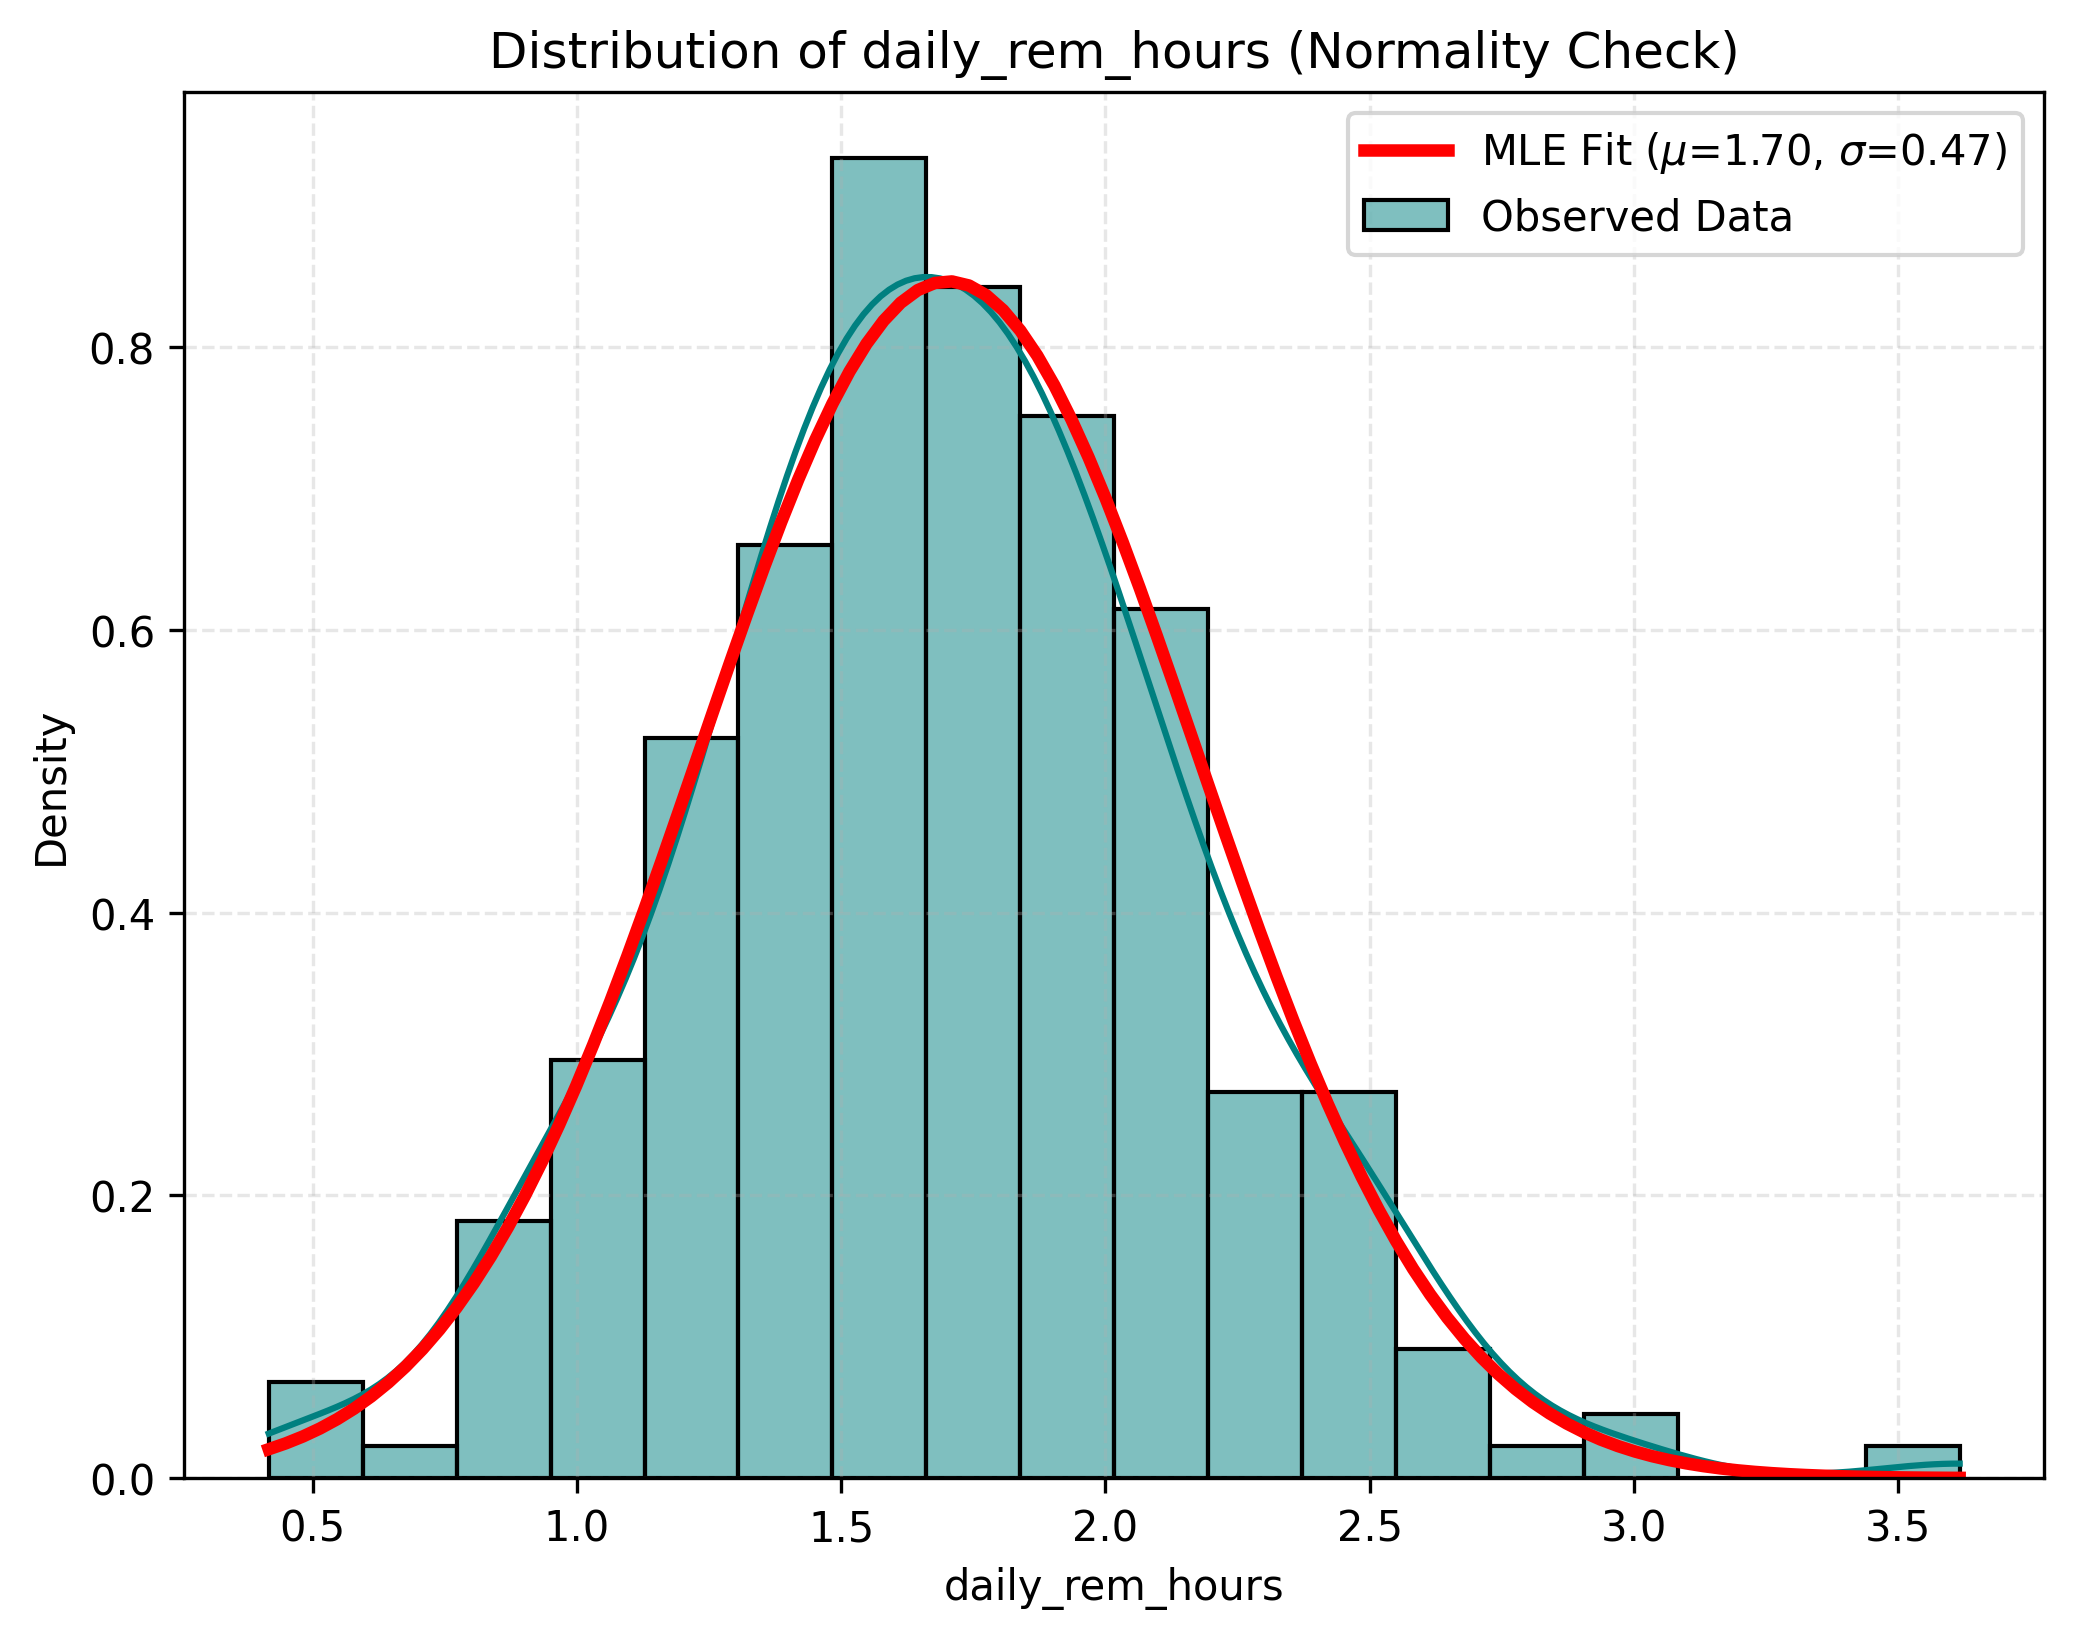
\includegraphics[width=0.85\linewidth]{dist_daily_rem_hours_MLE.png}
    \caption{Distribution of Daily REM Hours with MLE Normal Fit.}
    \label{fig:hist}
\end{figure}

To further assess outliers and spread, we examined the boxplot in Fig. \ref{fig:box}. The plot confirms the symmetry of the data, with the median centrally located within the interquartile range and minimal outliers.

\begin{figure}[H]
    \centering
    % Updated filename
    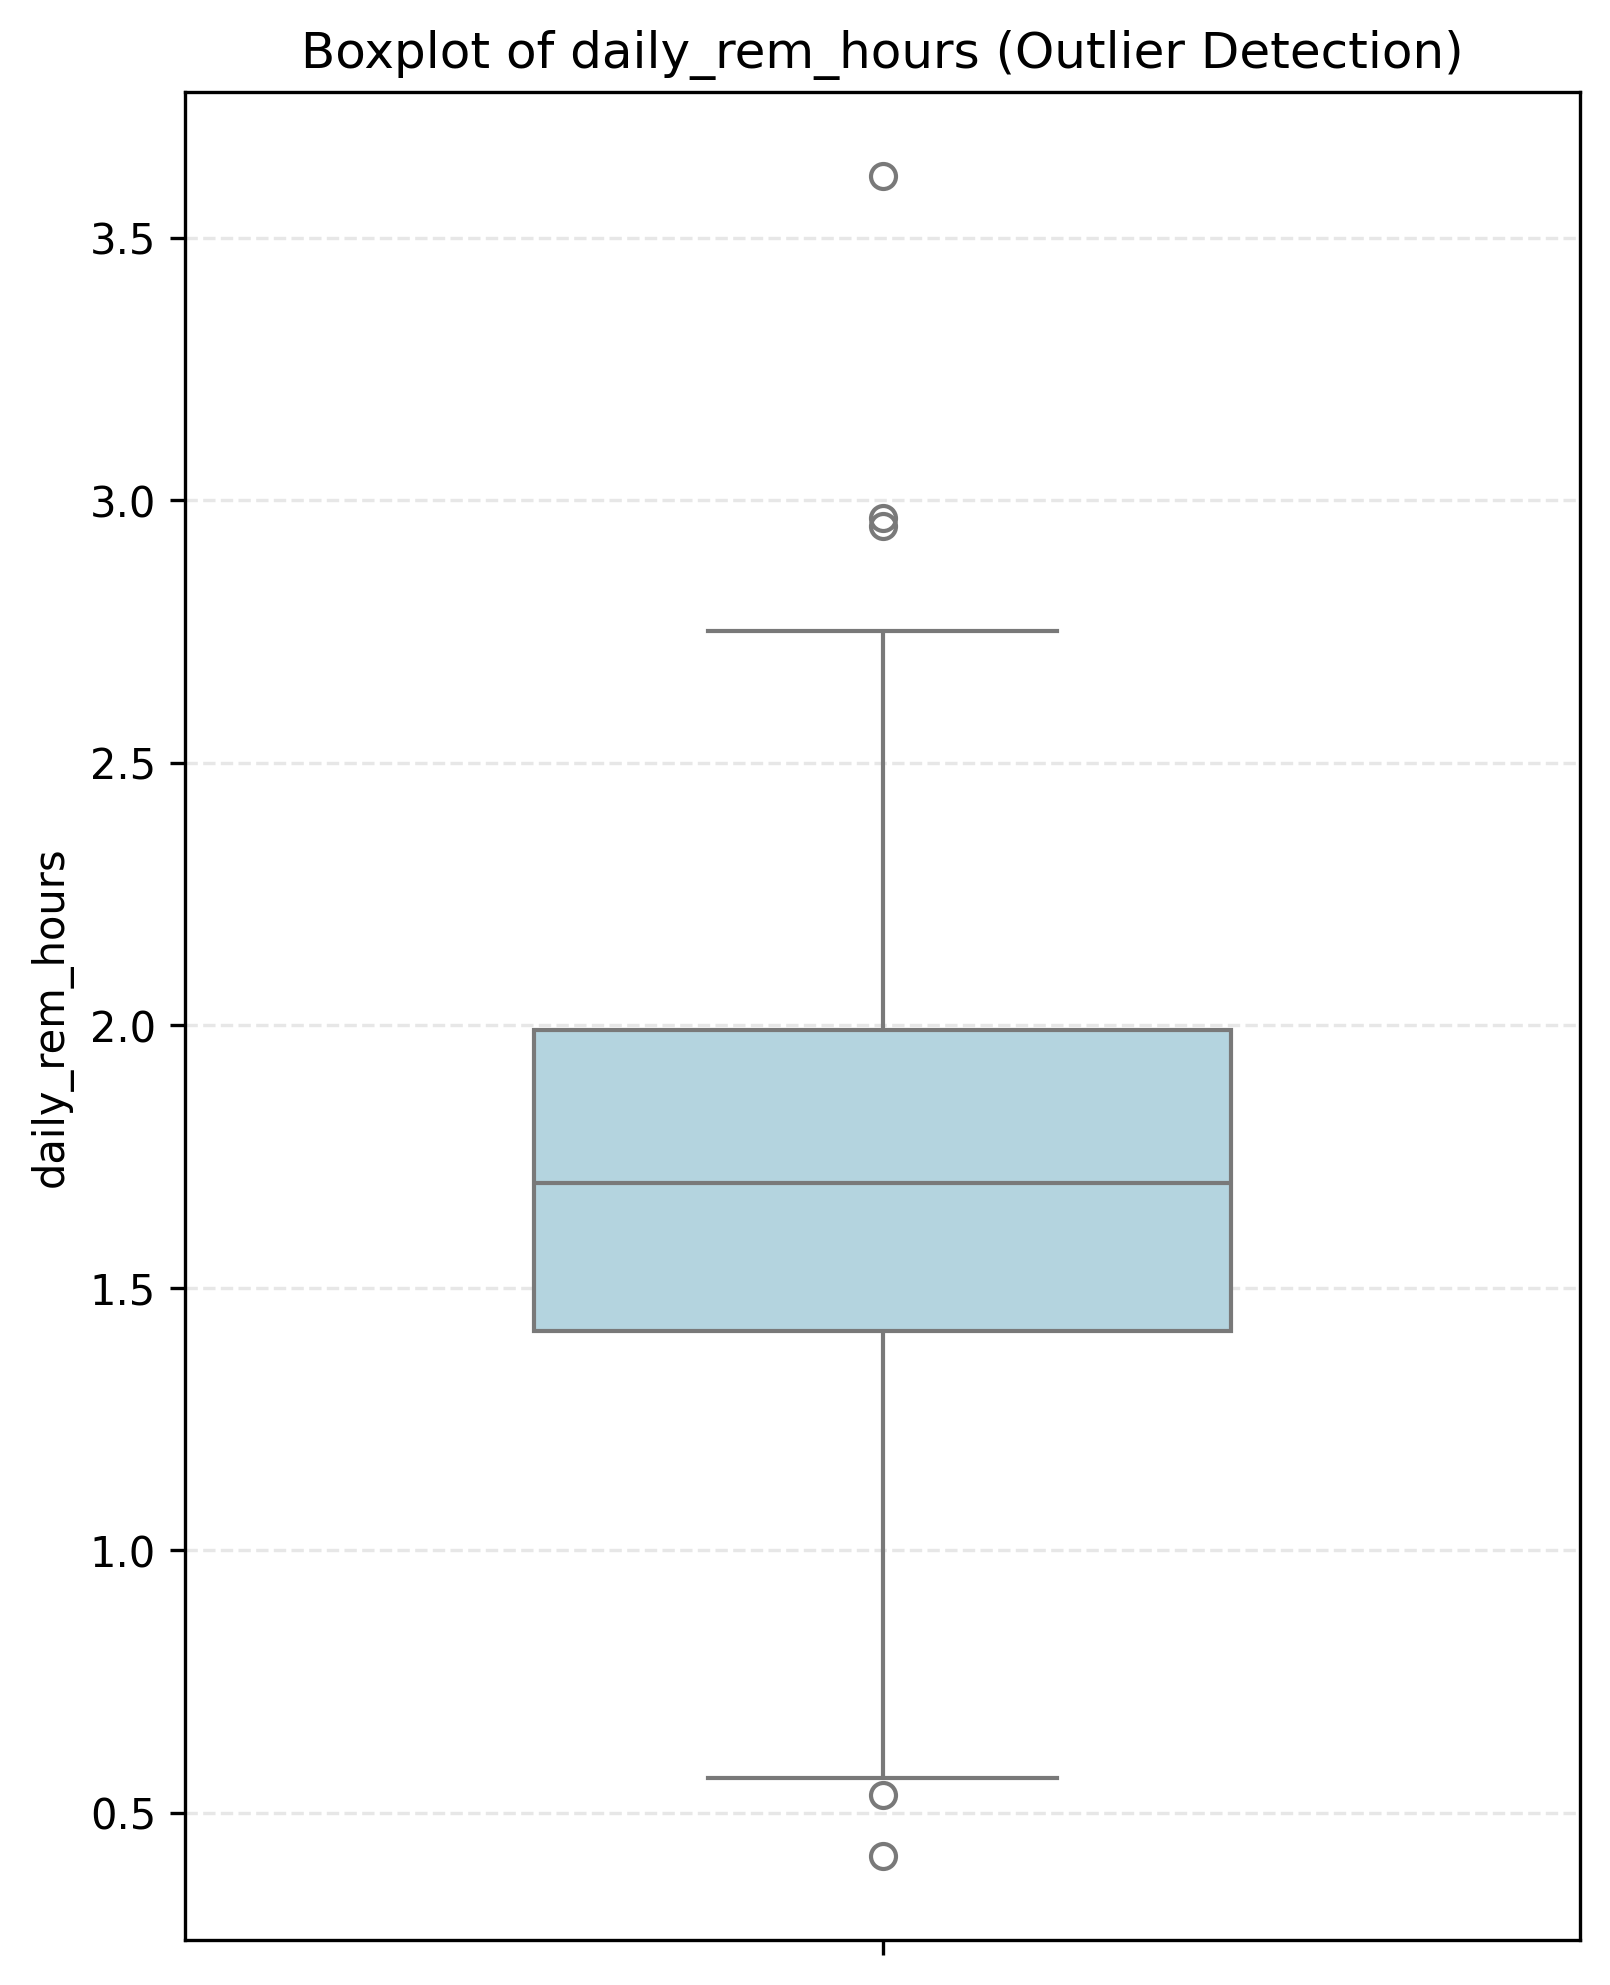
\includegraphics[width=0.6\linewidth]{boxplot_daily_rem_hours.png}
    \caption{Boxplot of Daily REM Sleep Hours.}
    \label{fig:box}
\end{figure}

\subsection{Correlation Analysis}
Fig. \ref{fig:scatter} illustrates the relationship between daily steps and REM sleep. A slight upward trend is visible, suggesting a positive correlation.

\begin{figure}[H]
    \centering
    % Updated filename
    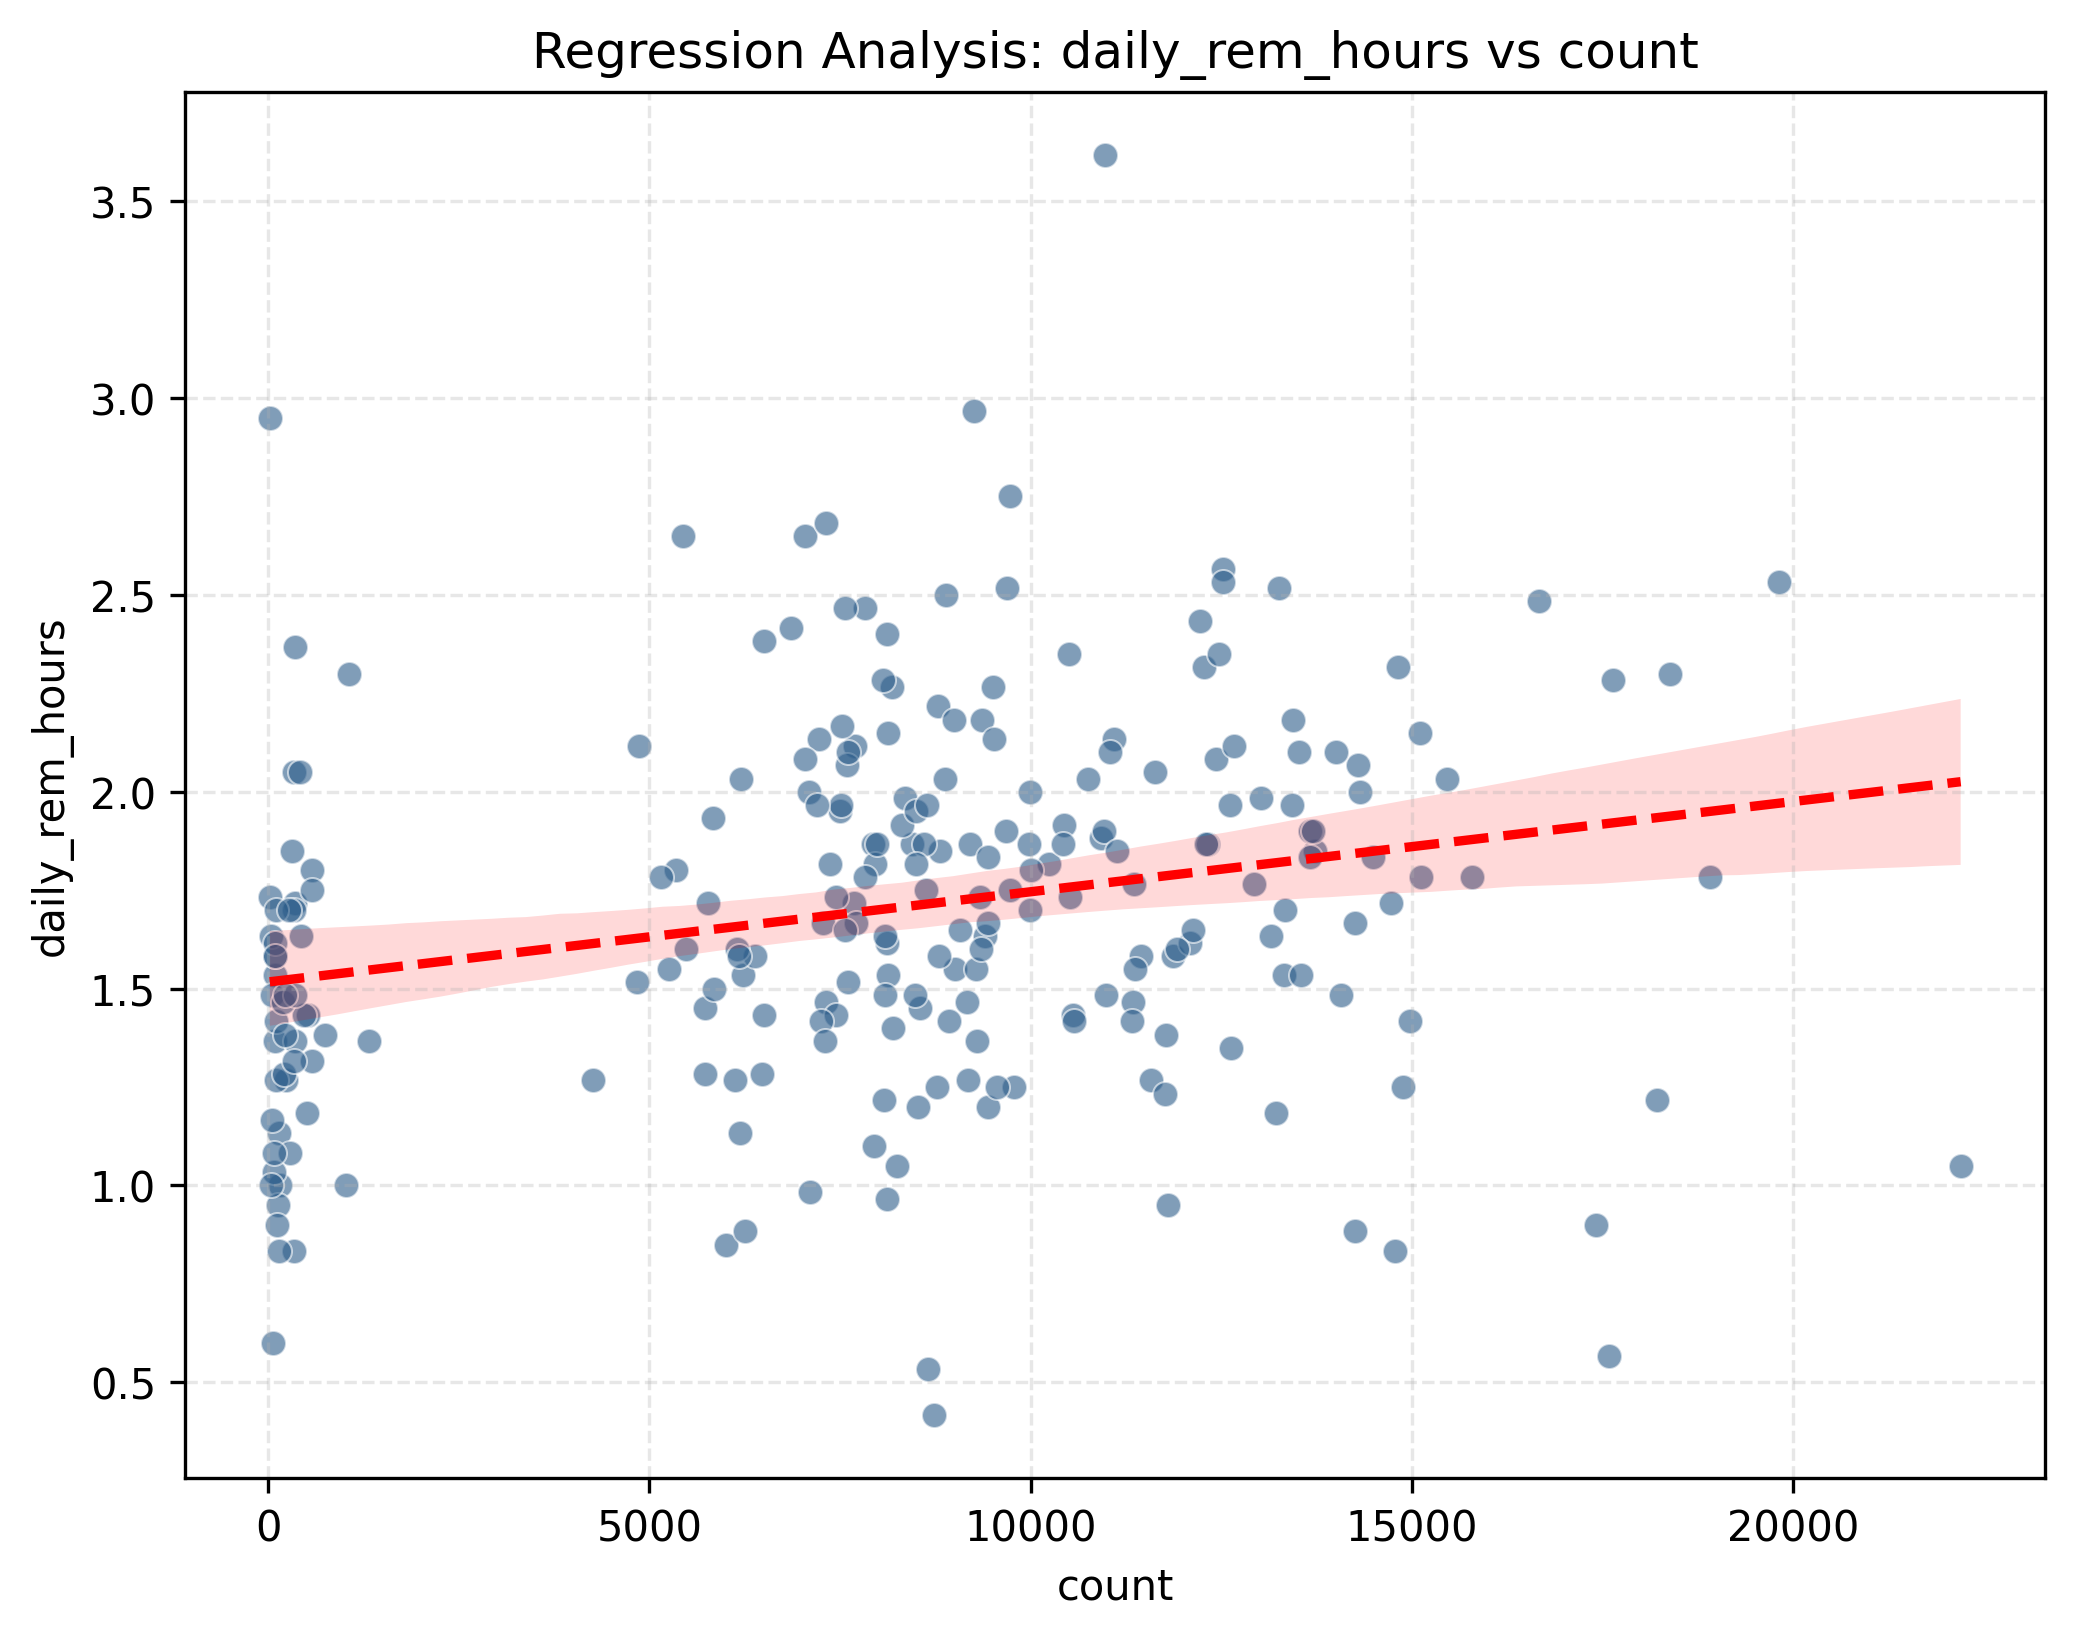
\includegraphics[width=0.85\linewidth]{scatter_daily_rem_hours_vs_count.png}
    \caption{Scatter Plot of REM Sleep vs. Daily Step Count with Regression Line.}
    \label{fig:scatter}
\end{figure}

\subsection{Temporal and Behavioral Patterns}
To investigate the impact of academic and work schedules on sleep architecture, we extended the exploratory analysis to include temporal trends.

\subsubsection{Weekly Cycles (Social Jetlag)}
A distinct weekly cycle was observed, characteristic of "Social Jetlag." As shown in Table \ref{tab:weekday_stats}, Mondays exhibit the lowest mean sleep (6.37 h) and REM duration (1.39 h). 

This reduction can be attributed to behavioral "bedtime procrastination" on Sunday nights, a voluntary delay of sleep intended to psychologically extend the weekend and avoid the onset of the work week (often referred to as "Monday Syndrome"), resulting in curtailed rest despite the lack of a forced wake-up time. In contrast, Saturdays show a compensatory "rebound" effect, with the mean sleep duration peaking at 9.11 hours.

\begin{table}[h]
\centering
\caption{Sleep Statistics by Weekday (Hours)}
\label{tab:weekday_stats}
\begin{tabular}{@{}lccccc@{}}
\toprule
 & & \multicolumn{2}{c}{Total Sleep} & \multicolumn{2}{c}{REM Sleep} \\
Day & \textbf{N} & Mean & Std & Mean & Std \\ \midrule
Monday    & 47 & 6.37 & 0.74 & 1.39 & 0.36 \\
Tuesday   & 44 & 6.73 & 0.84 & 1.60 & 0.43 \\
Wednesday & 39 & 6.77 & 0.88 & 1.72 & 0.41 \\
Thursday  & 48 & 6.79 & 0.82 & 1.76 & 0.36 \\
Friday    & 45 & 6.87 & 0.81 & 1.76 & 0.45 \\
Saturday  & 12 & 9.11 & 1.05 & 2.41 & 0.56 \\
Sunday    & 13 & 7.96 & 1.49 & 2.05 & 0.52 \\ \bottomrule
\end{tabular}
\end{table}

Notably, Sundays exhibit the highest standard deviation in total sleep ($\sigma = 1.49$). This variance suggests that Sunday serves as a transitional period with irregular sleep behaviors, likely influenced by varying Monday schedules.

\subsubsection{Physical Activity Patterns}
To understand the drivers of the observed sleep variance, we analyzed daily step counts across the same period.

Table \ref{tab:step_stats} summarizes the weekly activity cycle. A clear behavioral pattern emerges: Weekdays (Monday--Friday) exhibit consistently higher mean step counts ($\mu > 8,700$), consistent with the commute to university classes (Tuesday). In contrast, Sundays show significantly reduced physical activity ($\mu \approx 2,458$), aligning with the "rest day" hypothesis and the potential measurement bias (reduced phone carriage).

\begin{table}[h]
\centering
\caption{Step Count Statistics by Weekday}
\label{tab:step_stats}
\begin{tabular}{@{}lccc@{}}
\toprule
Day & N & Mean Steps & Std Dev \\ \midrule
Monday    & 62 & 8,754 & 2,924 \\
Tuesday   & 62 & 9,739 & 4,278 \\
Wednesday & 63 & 9,264 & 3,831 \\
Thursday  & 63 & 9,316 & 3,064 \\
Friday    & 63 & 9,581 & 3,267 \\
Saturday  & 62 & 7,059 & 5,830 \\
Sunday    & 61 & 2,458 & 4,814 \\ \bottomrule
\end{tabular}
\end{table}

We also examined monthly trends in physical activity in Table \ref{tab:combined_stats}. The data indicates an increasing trend in activity towards the end of 2025, with December 2025 recording the highest mean step count ($\mu = 10,715$). This peak is attributed to a behavioral shift in the subject's commute, specifically the decision to walk directly to the tram station to avoid inconsistent bus wait times.

\subsubsection{Long-Term Trends}
Monthly analysis (Table \ref{tab:combined_stats}) reveals fluctuations in sleep duration. Notably, a dip in REM sleep duration is observed in May 2025 ($\mu=1.47$). 

\begin{figure}[H]
    \centering
    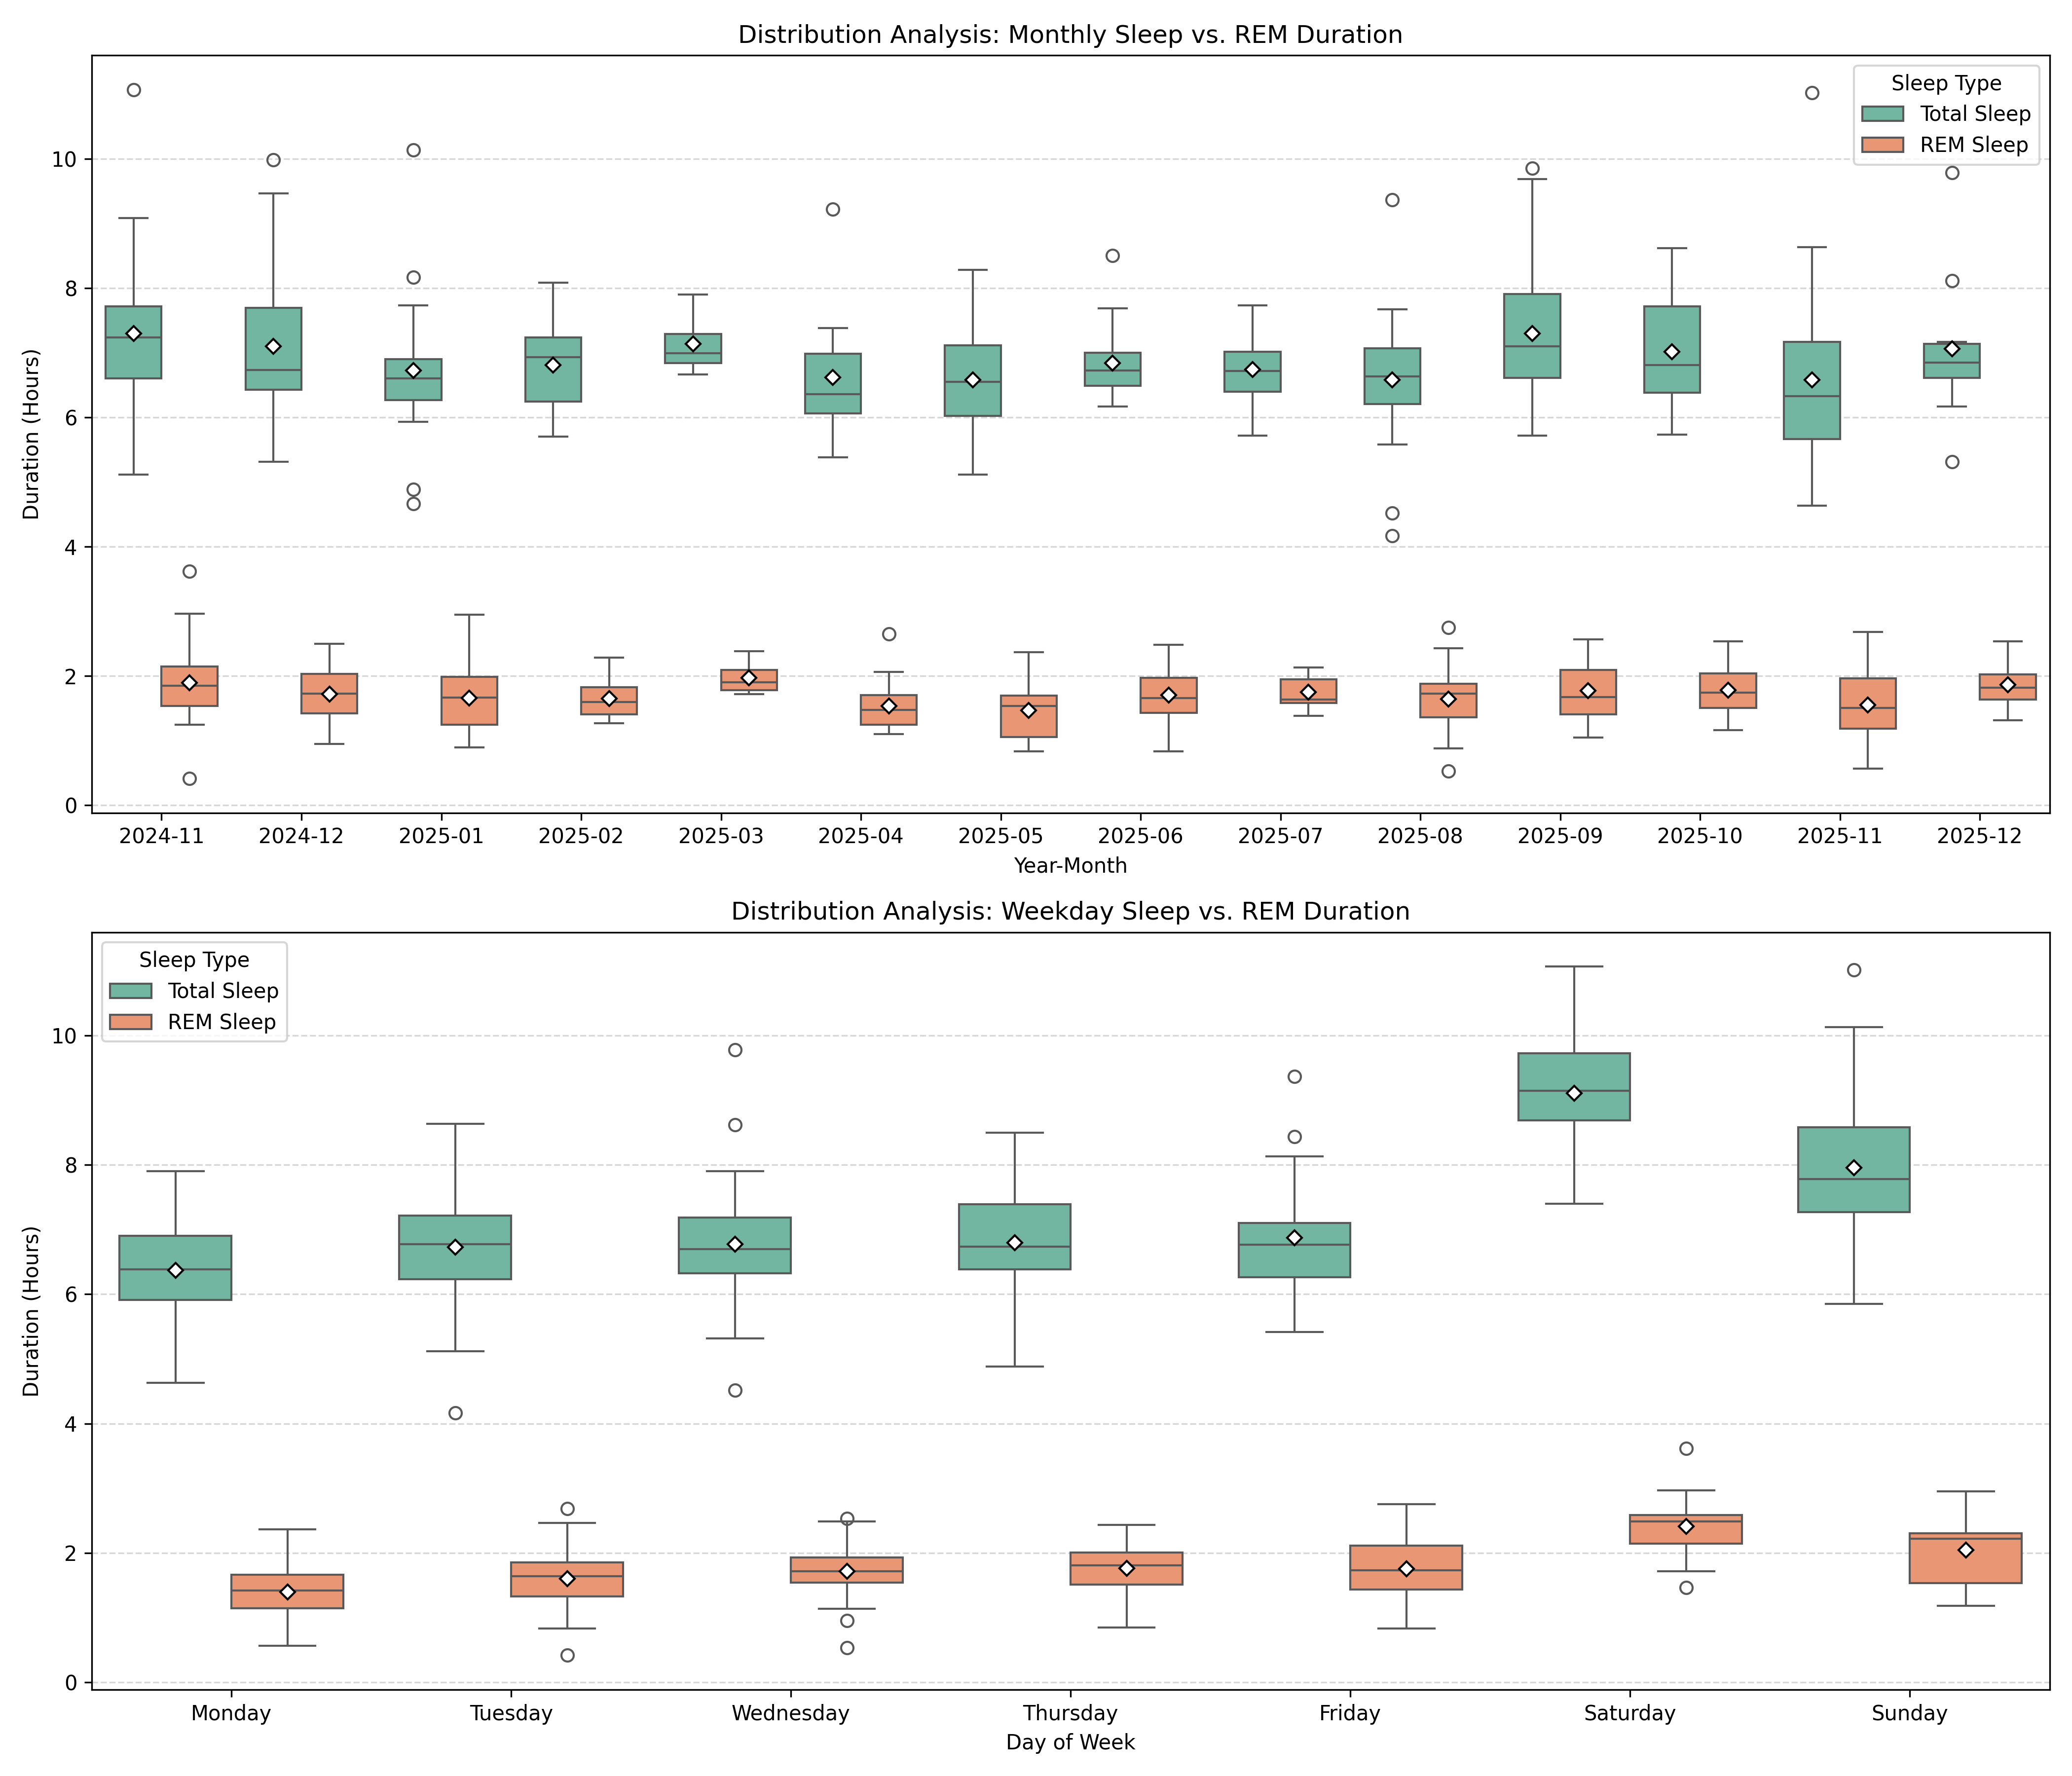
\includegraphics[width=0.95\linewidth]{distribution_stats_analysis.png}
    \caption{Temporal Sleep Analysis: Showing monthly and weekday trends, respectively.}
    \label{fig:temporal}
\end{figure}

\begin{figure}[H]
    \centering
    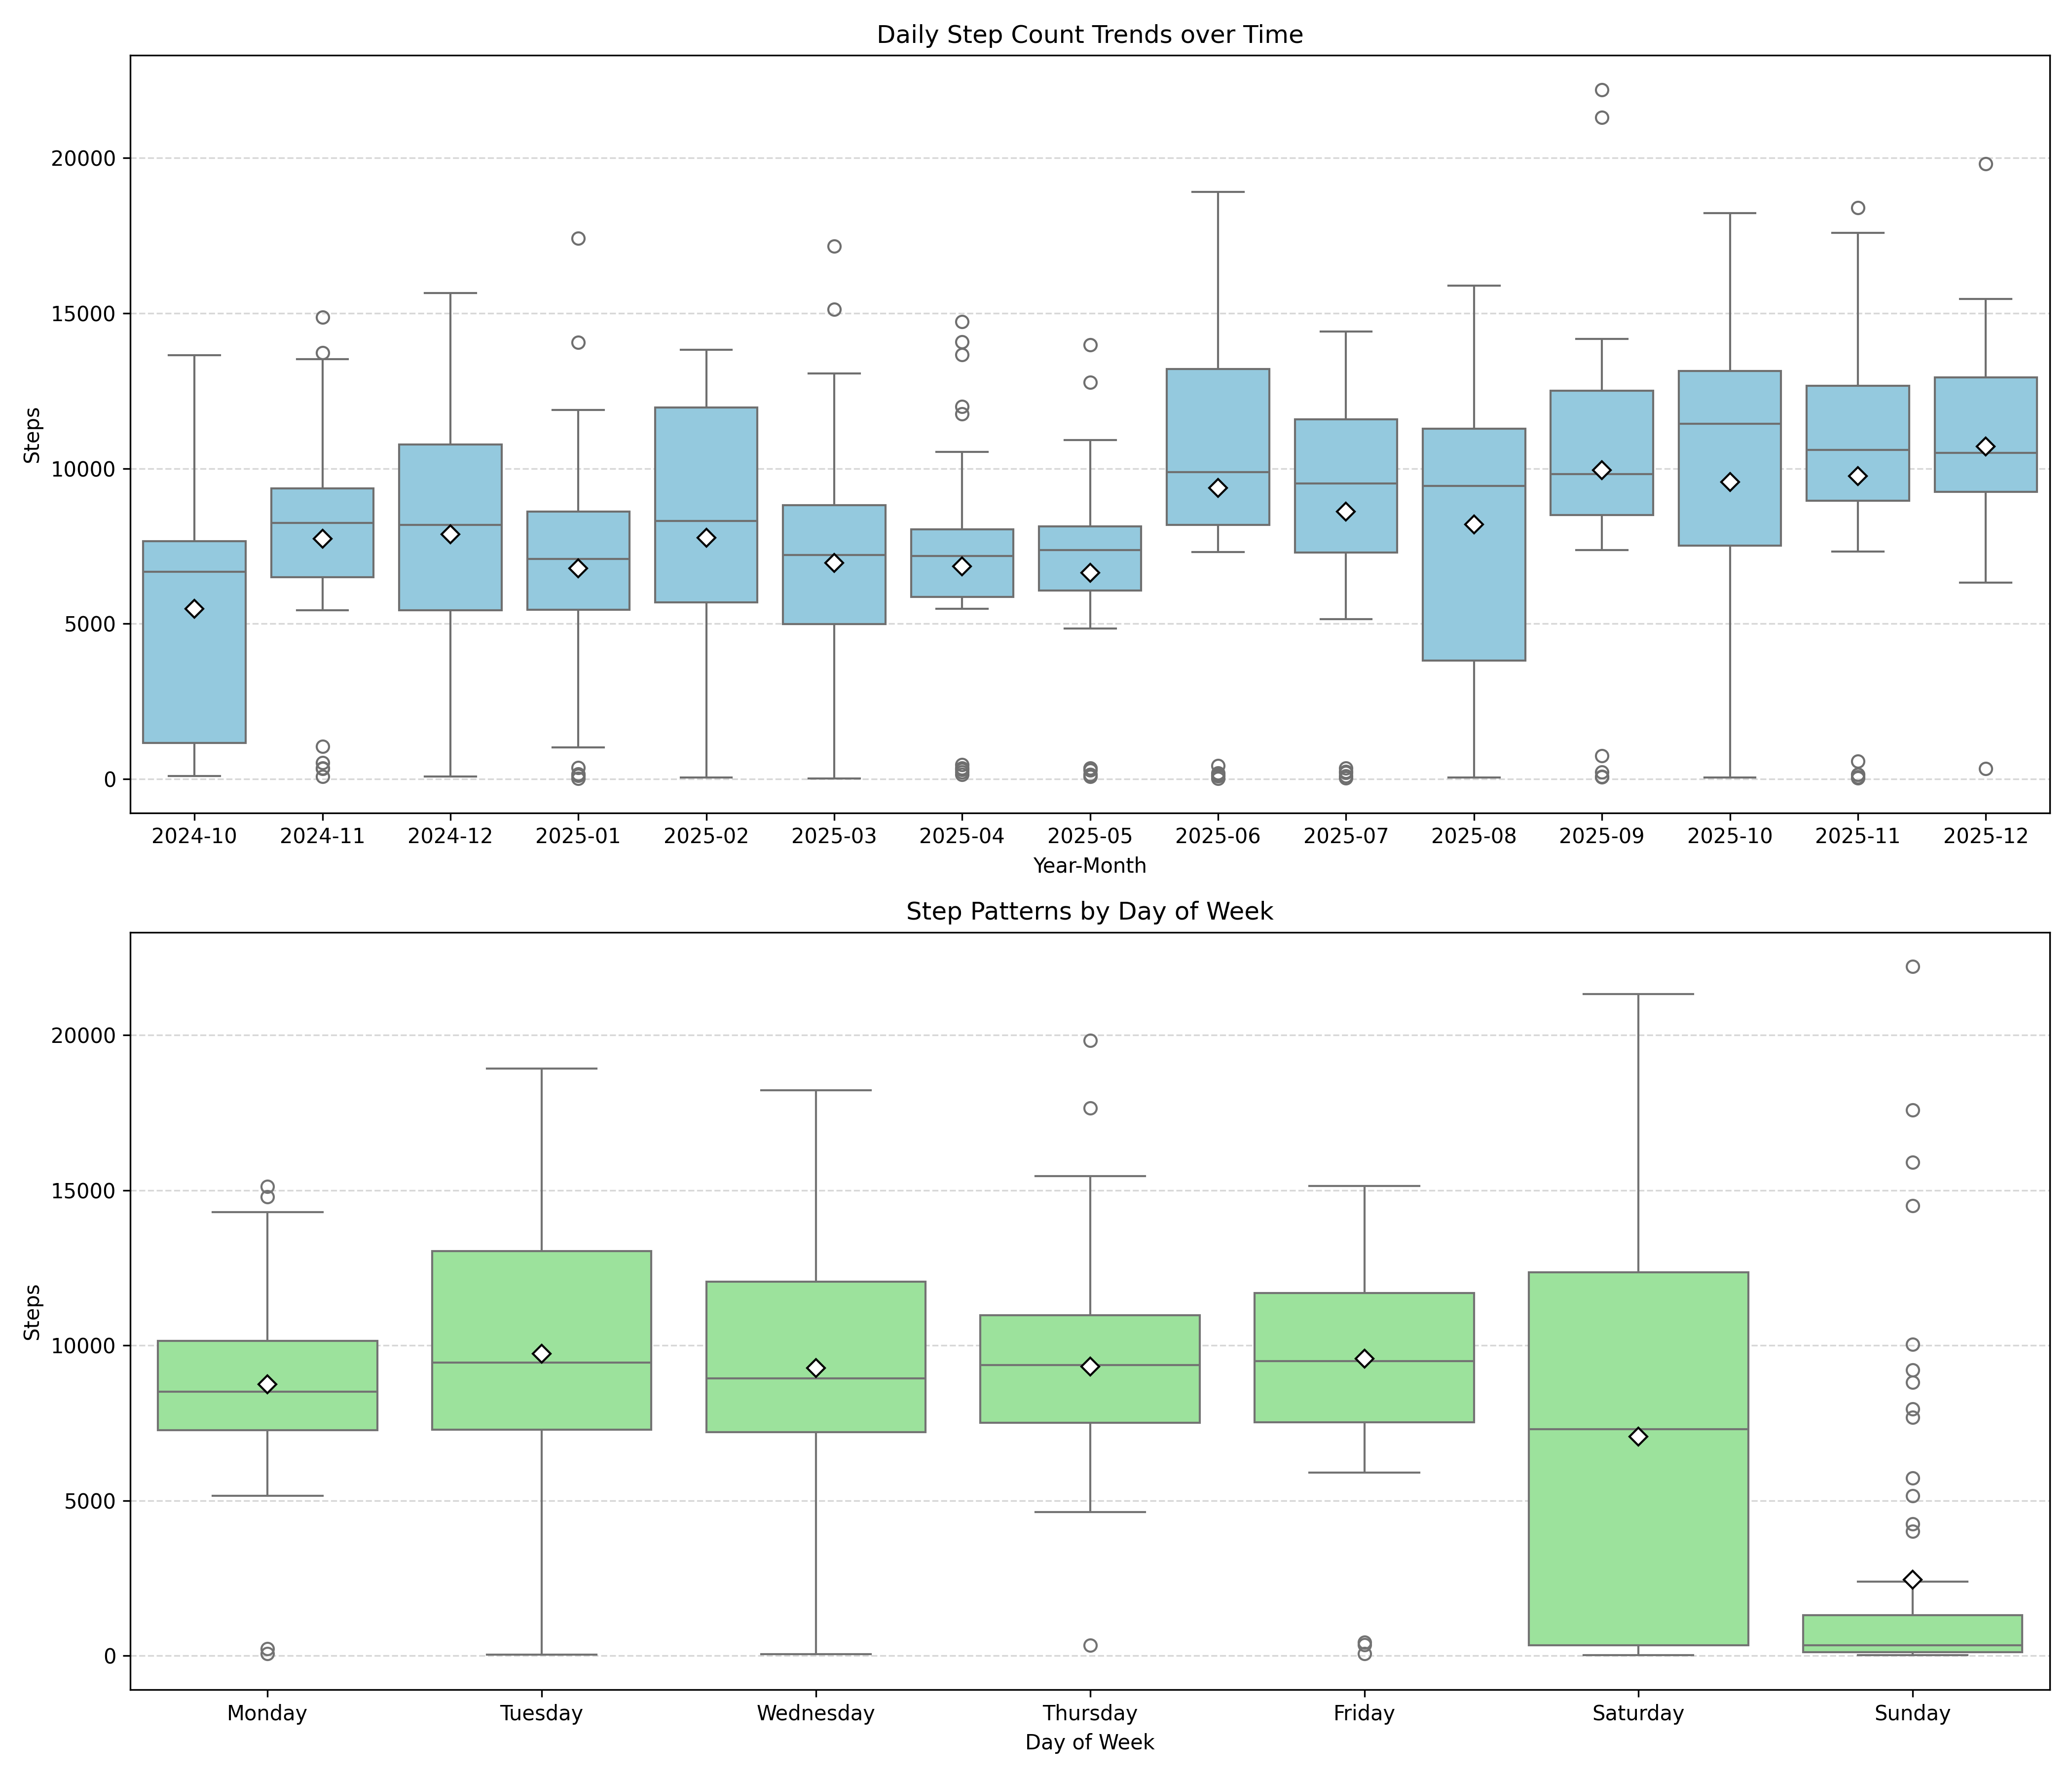
\includegraphics[width=0.95\linewidth]{step_analysis.png}
    \caption{Step Count Analysis: Showing monthly and weekday trends, respectively.}
    \label{fig:steps}
\end{figure}

\section{Determining the Underlying Distribution}
Based on the EDA, the Normal distribution was proposed as the underlying model for daily REM sleep.

\subsection{Parameter Estimation}
We estimated the parameters $\mu$ (mean) and $\sigma$ (standard deviation) using three methods:

\subsubsection{Maximum Likelihood Estimation}
The MLE parameters were calculated as:
\[ \hat{\mu}_{MLE} = 1.7023, \quad \hat{\sigma}_{MLE} = 0.4712 \]

\subsubsection{Method of Moments}
For a Normal distribution, MoM estimates coincide with the sample moments:
\[ \hat{\mu}_{MoM} = 1.7023, \quad \hat{\sigma}_{MoM} = 0.4712 \]

\subsubsection{Bayesian Estimation}
We applied a Bayesian approach using a conjugate prior. Based on general health recommendations, we established a prior belief of $\mu_0 = 1.5$ with uncertainty $\tau = 0.5$. The posterior mean was calculated as:
\begin{equation}
    \hat{\mu}_{Bayes} = \frac{\sigma^2 \mu_0 + n \tau^2 \bar{x}}{n \tau^2 + \sigma^2} = 1.7016
\end{equation}
The Bayesian estimate converges closely to the MLE due to the dominance of the likelihood ($N=247$) over the prior.

\section{Goodness-of-Fit and Hypothesis Testing}

\subsection{Goodness-of-Fit Test}
To formally verify the assumption of Normality, we performed the Kolmogorov-Smirnov (KS) test.
\begin{itemize}
    \item \textbf{$H_0$:} The data follows a Normal distribution.
    \item \textbf{Result:} $D = 0.0438$, $p\text{-value} = 0.7143$.
\end{itemize}
Since $p > 0.05$, we fail to reject the null hypothesis. This indicates that the data does not significantly deviate from a Normal distribution. Therefore, the assumption of normality is considered valid for the subsequent parametric analyses.

\subsection{Hypothesis Testing on the Mean}
We aimed to test if the subject's average REM sleep differs significantly from the benchmark of 1.5 hours.
\[ H_0: \mu = 1.5, \quad H_1: \mu \neq 1.5 \]
Since the data is Normal, we used a one-sample t-test.
\begin{itemize}
    \item \textbf{T-Statistic:} 6.7334
    \item \textbf{P-Value:} $< 0.0001$
\end{itemize}
The result is statistically significant. We reject $H_0$ and conclude that the subject averages significantly more REM sleep than the 1.5 hour benchmark.

\section{Regression Analysis}
To quantify the relationship between daily activity and REM sleep, we fitted a simple linear regression model:
\[ Y = \beta_0 + \beta_1 X + \epsilon \]
where $Y$ is \texttt{daily\_rem\_hours} and $X$ is \texttt{count}.

\subsection{Model Results}
The regression output is summarized below:
\begin{itemize}
    \item \textbf{Intercept ($\beta_0$):} $1.5169$
    \begin{itemize}
        \item $t\text{-statistic} = 26.799$
        \item $p\text{-value} < 0.001$
    \end{itemize}
    \item \textbf{Slope ($\beta_1$):} $2.29 \times 10^{-5}$
    \begin{itemize}
        \item $t\text{-statistic} = 3.825$
        \item $p\text{-value} < 0.001$
    \end{itemize}
    \item \textbf{Model Fit:} $R^2 = 0.056$, $F = 14.63$ ($p < 0.001$)
\end{itemize}

\subsection{Interpretation}
The slope coefficient yields a $t$-statistic of 3.825, which corresponds to a $p$-value of effectively zero ($< 0.001$). This allows us to reject the null hypothesis ($\beta_1 = 0$) and conclude that there is a statistically significant positive relationship between step count and REM sleep.

However, the low $R^2$ value (0.056) indicates that daily steps explain only 5.6\% of the variance in REM sleep. While the relationship is significant, the effect size is modest, suggesting that sleep architecture is multifactorial and heavily influenced by unobserved variables.

\section{Conclusion}
This study successfully applied statistical inference to personal health data. We confirmed that daily REM sleep duration follows a Normal distribution. Hypothesis testing showed the subject averages significantly more REM sleep than the standard benchmark. Finally, regression analysis established a positive, statistically significant link between daily step count and REM sleep, confirming the initial hypothesis that daily activity impacts sleep quality, though the effect size is modest.

\section*{Acknowledgement}
Google Gemini is used for assistance in generating the Python syntax for the data visualizations and mathematical LaTeX notations presented in this report. All data collection, statistical methodology, and interpretation of findings are the original work of the author.

\bibliographystyle{IEEEtran}
% References would go here if using a .bib file
% \bibliography{references}

\end{document}